\documentclass[twoside, a4paper]{article}

\usepackage[utf8]{inputenc}
\usepackage{dblfloatfix}
\usepackage{subcaption}
\usepackage{float}
\usepackage[backend=biber, maxbibnames=3, style=nature, autocite=inline]{biblatex}
\usepackage[polish]{babel}
\usepackage[T1]{fontenc}
\usepackage{fancyhdr}
\usepackage{titlesec}
\usepackage{blindtext}
\usepackage{gensymb}
\usepackage{cuted}
\usepackage{tikz}
\usepackage[most]{tcolorbox}
\usepackage[columnsep = 0.7cm,
	        lmargin = 0.6in,
	        rmargin = 0.6in,
	        tmargin = 0.5in,
	        bmargin = 0.65in,
	        headsep = \baselineskip]{geometry}

\addbibresource{$BIB}

% Custom commands
\newcommand*\circled[1]{\tikz[baseline=(char.base)]{
            \node[shape=circle,draw,inner sep=2pt, color = orange!90!white] (char) {#1};}}

% Section Formatting
\titleformat{\section}
{\sc \bfseries \Large}
{}
{0em}
{}[\titlerule]

\titleformat{\subsection}
{\bfseries \large}
{}
{0em}
{}

\titleformat{\subsubsection}
{\bfseries}
{}
{0em}
{}

\setlength{\parindent}{0in}

% Box formatting
\tcbset{sharp corners, colback=white, enhanced, boxrule = 1pt, coltitle = orange!90!white, colbacktitle = orange!15!white, colframe= black!50!white}

\pagestyle{fancy}
\fancyhf{}
\fancyhead[RE, LO]{Szkoła Główna Gospodarstwa Wiejskiego}
\fancyhead[LE, RO]{Biotechnologia, semerstr V}
\fancyfoot[RE, LO]{Jakub J. Guzek}
\fancyfoot[LE, RO]{\thepage}
\fancyfoot[CE,CO]{Inżynieria Genetyczna}
\renewcommand{\footrulewidth}{0.05pt}

\begin{document}

	{\sc \bfseries \LARGE \fontfamily{phv}\selectfont Otrzymanie pomidora odpornego na infekcję \textit{Phytophthora capsici} metodą CRISPR/Cas9 -- Suplement } \vspace{\baselineskip}

{\bfseries \large Jakub J. Guzek}

{Szkoła Główna Gospodarstwa Wiejskiego. Biotechnologia, Semestr V, nr. albumu: 195528}\vspace{\baselineskip}

\hrule

	\textbf{\textsf{Choroby roślin powodują co roku ogromne straty gospodarcze. Nierzadko cała uprawa zostaje zmarnowana na skutek zakażenia patogenem. Rozwiązaniem tego problemu jest otrzymywanie odmian roślin odpornych na działanie tych patogenów. Jednak tradycyjne metody selekcjonowania nowych odmian zawodzą i nie dają długotrwałych rezultatów w wypadku niektórych chorób. Współcześnie dzięki metodom transformacji roślin i ukierunkowanej mutagenezy (genome-editing) możliwe jest otrzymanie odpornych odmian łatwiej i skuteczniej niż wcześniej. W tym projekcie opisuję proces otrzymywania odmiany pomidora odpornej na infekcję \textit{Phytophthora capsici}, przy użyciu transformacji roślin za pomocą \textit{A. tumefaciens} i metody edycji genomu CRISPR-Cas9}}\vspace{\baselineskip}

\hrule

 \begin{figure}[h]
	 \centering
	 \includegraphics[width=\textwidth]{./figures/pPZP200-CRISPR.png}
	 \caption{Schemat konstruktu AtU6-sgRNA-2x35S-Cas9\protect\footnotemark}
\end{figure}

\pagebreak

\begin{table}
	\centering
	\caption{Wybrane sekwencje sgRNA (Na podstawie: CRISPR-P)}
	\includegraphics[width=0.95\textwidth]{./figures/gRNA.png}
\end{table}

\begin{figure}[h]
	\centering
	\begin{subfigure}[t]{0.45\textwidth}
		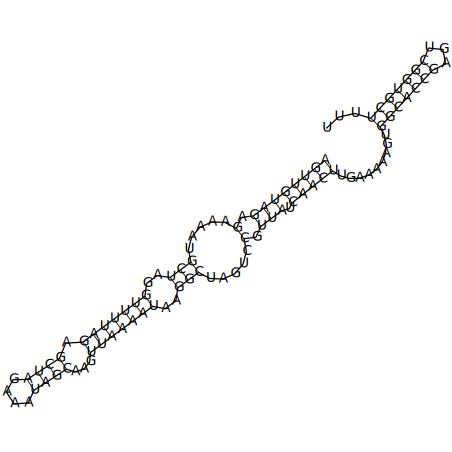
\includegraphics[width=\textwidth]{./figures/gRNA-ekson2.pdf}
		\caption{}
	\end{subfigure}
	\hfill
	\begin{subfigure}[t]{0.45\textwidth}
		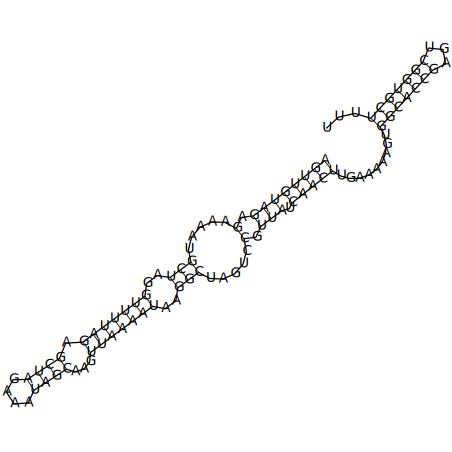
\includegraphics[width=\textwidth]{./figures/gRNA-ekson2.pdf}
		\caption{}
	\end{subfigure}
	\caption{Struktury drugodzędowe (a) sgRNA targetujacego ekson 2 DMR6 i (b) sgRNA targetującego ekson 3 genu DMR6. Otrzymane za pomocą narzędzia CRISPR-P}
\end{figure}

\nocite{Lei2014}
\footnotetext{Schemat utworzony przy użyciu narzędzia \textsf{Angluar Plasmid}}

\printbibliography

\end{document}
